% Offline Qwen3-ASR vs this release's causal streaming execution.
% Visual language follows Fig. 2 of the Qwen3-ASR technical report
% (arXiv:2601.21337); redrawn, not copied.
% Compile: lualatex offline_vs_causal.tex ; export: pdftocairo -svg
\documentclass[tikz,border=10pt]{standalone}
\usetikzlibrary{arrows.meta,calc,decorations.pathreplacing,positioning}
\renewcommand{\familydefault}{\sfdefault}

\definecolor{boxgray}{HTML}{D9D9D9}
\definecolor{boxedge}{HTML}{8A8A8A}
\definecolor{tokyellow}{HTML}{F6CD61}
\definecolor{tokyellowmute}{HTML}{F8E3AC}
\definecolor{tokteal}{HTML}{7FD6C2}
\definecolor{toktealmute}{HTML}{C8EDE4}
\definecolor{labelpurple}{HTML}{6C4FD8}
\definecolor{inkgray}{HTML}{5A5A5A}
\definecolor{accent}{HTML}{0A66A3}
\definecolor{accentlight}{HTML}{D7E7F3}
\definecolor{mute}{HTML}{C9C9C9}

\newcommand{\waveform}[3]{% x0, length, opacity
  \begin{scope}[opacity=#3]
  \foreach \i in {0,...,#2}{
    \pgfmathsetmacro{\h}{0.10 + 0.16*abs(sin(\i*47) * sin(\i*13+40)) + 0.10*abs(sin(\i*89))}
    \draw[line width=0.55pt, inkgray] ({#1 + \i*0.066}, -\h) -- ({#1 + \i*0.066}, \h);
  }
  \end{scope}
}

\begin{document}
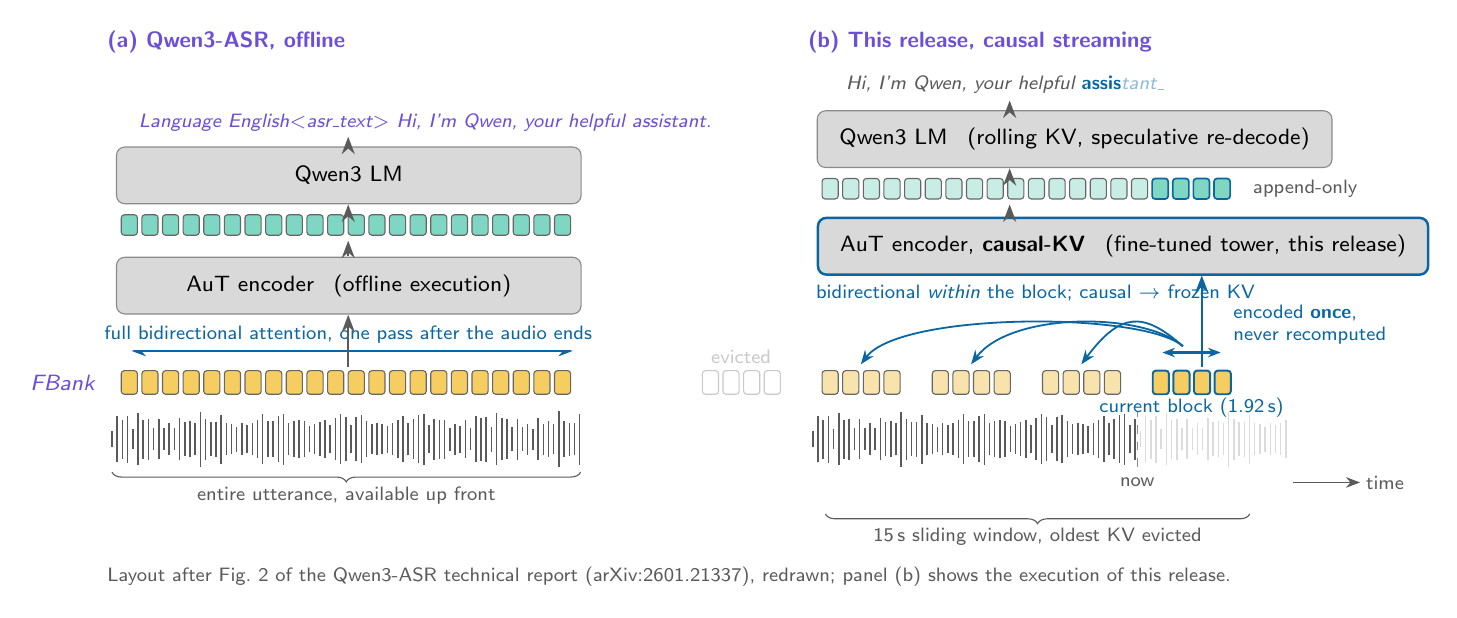
\begin{tikzpicture}[
  font=\footnotesize,
  bigbox/.style={rounded corners=3pt, draw=boxedge, fill=boxgray,
                 minimum height=0.72cm, inner xsep=8pt},
  tok/.style={rounded corners=1.1pt, minimum width=0.205cm, minimum height=0.30cm,
              inner sep=0, draw=black!60, line width=0.4pt},
  plbl/.style={labelpurple, font=\footnotesize\itshape, inner sep=1pt},
  glbl/.style={inkgray, font=\scriptsize, inner sep=1pt},
  flow/.style={-{Stealth[length=2.2mm]}, inkgray, line width=0.9pt},
  attn/.style={-{Stealth[length=1.8mm]}, accent, line width=0.65pt},
]

% =========================== LEFT: offline ===========================
\begin{scope}[local bounding box=leftpanel]
  \node[plbl, anchor=west] at (-0.1, 5.05) {\textbf{(a) Qwen3-ASR, offline}};

  % waveform: whole utterance present
  \waveform{0}{90}{1.0}
  \draw[decorate, decoration={brace, mirror, amplitude=3.5pt}, inkgray]
    (0,-0.42) -- (5.95,-0.42) node[midway, below=4pt, glbl] {entire utterance, available up front};

  % fbank tokens, all at once
  \foreach \i in {0,...,21}{ \node[tok, fill=tokyellow] at (0.22+\i*0.262, 0.72) {}; }
  \node[plbl, anchor=east] at (-0.18, 0.72) {FBank};

  % full bidirectional attention glyph
  \draw[{Stealth[length=1.8mm]}-{Stealth[length=1.8mm]}, accent, line width=0.8pt]
    (0.25, 1.12) -- (5.85, 1.12);
  \node[glbl, accent, fill=white, inner sep=2.5pt] at (3.0, 1.33) {full bidirectional attention, one pass after the audio ends};

  % encoder box
  \node[bigbox, minimum width=5.9cm, anchor=west] (enc) at (0.05, 1.95) {AuT encoder \, (offline execution)};
  \draw[flow] (3.0, 0.92) -- (3.0, 1.58);

  % hidden tokens
  \foreach \i in {0,...,21}{ \node[tok, fill=tokteal, minimum height=0.26cm] at (0.22+\i*0.262, 2.72) {}; }
  \draw[flow] (3.0, 2.32) -- (3.0, 2.52);

  % LM box + output
  \node[bigbox, minimum width=5.9cm, anchor=west] (lm) at (0.05, 3.35) {Qwen3 LM};
  \draw[flow] (3.0, 2.92) -- (3.0, 2.98);
  \node[plbl, anchor=west, font=\scriptsize\itshape] at (0.3, 4.02)
    {Language English\textless asr\_text\textgreater\ Hi, I'm Qwen, your helpful assistant.};
  \draw[flow] (3.0, 3.72) -- (3.0, 3.84);
\end{scope}

% =========================== RIGHT: causal ===========================
\begin{scope}[xshift=8.9cm, local bounding box=rightpanel]
  \node[plbl, anchor=west] at (-0.1, 5.05) {\textbf{(b) This release, causal streaming}};

  % waveform: past solid, future faded
  \waveform{0}{62}{1.0}
  \waveform{4.16}{28}{0.22}
  \draw[-{Stealth[length=1.8mm]}, inkgray] (6.1, -0.55) -- (6.95, -0.55) node[glbl, right=1pt] {time};
  \draw[inkgray!70, line width=0.5pt, dashed] (4.12, -0.35) -- (4.12, 0.35);
  \node[glbl] at (4.12, -0.55) {now};

  % fbank tokens grouped in blocks of 5 (one block = 1.92 s)
  % evicted block
  \foreach \i in {0,...,3}{ \node[tok, fill=white, draw=mute] at (-1.30+\i*0.262, 0.72) {}; }
  \node[glbl, text=mute] at (-0.91, 1.05) {evicted};
  % three frozen blocks + current block
  \foreach \b/\xs in {0/0.22, 1/1.62, 2/3.02}{
    \foreach \i in {0,...,3}{ \node[tok, fill=tokyellowmute] at (\xs+\i*0.262, 0.72) {}; }
  }
  \foreach \i in {0,...,3}{
    \node[tok, fill=tokyellow, draw=accent, line width=0.7pt] at (4.42+\i*0.262, 0.72) {};
  }
  \node[glbl, accent] at (4.81, 0.40) {current block (1.92\,s)};

  % intra-block bidirectional + causal arrows to past blocks
  \draw[{Stealth[length=1.6mm]}-{Stealth[length=1.6mm]}, accent, line width=0.75pt]
    (4.44, 1.10) -- (5.18, 1.10);
  \foreach \xs in {0.61, 2.01, 3.41}{
    \draw[attn] (4.70, 1.18) .. controls (4.2, 1.62) and (\xs+0.5, 1.62) .. (\xs, 0.95);
  }
  \node[glbl, accent, anchor=west] at (0.0, 1.85) {bidirectional \emph{within} the block; causal $\rightarrow$ frozen KV};
  \draw[decorate, decoration={brace, mirror, amplitude=3.5pt}, inkgray]
    (0.16,-0.95) -- (5.55,-0.95) node[midway, below=4pt, glbl] {15\,s sliding window, oldest KV evicted};

  % encoder box
  \node[bigbox, minimum width=6.5cm, anchor=west, draw=accent, line width=0.9pt] (enc2) at (0.05, 2.45)
    {AuT encoder, \textbf{causal-KV} \, (fine-tuned tower, this release)};
  \draw[flow, accent] (4.94, 0.92) -- (4.94, 2.08);
  \node[glbl, accent, align=left, anchor=west] at (5.30, 1.45) {encoded \textbf{once},\\never recomputed};

  % hidden tokens: append-only
  \foreach \i in {0,...,15}{ \node[tok, fill=toktealmute, minimum height=0.26cm] at (0.22+\i*0.262, 3.18) {}; }
  \foreach \i in {16,...,19}{ \node[tok, fill=tokteal, draw=accent, line width=0.6pt, minimum height=0.26cm] at (0.22+\i*0.262, 3.18) {}; }
  \node[glbl, anchor=west] at (5.55, 3.18) {append-only};
  \draw[flow] (2.5, 2.82) -- (2.5, 2.98);

  % LM box + streaming output
  \node[bigbox, minimum width=6.5cm, anchor=west] (lm2) at (0.05, 3.81) {Qwen3 LM \, (rolling KV, speculative re-decode)};
  \draw[flow] (2.5, 3.38) -- (2.5, 3.44);
  \node[anchor=west, font=\scriptsize\itshape] at (0.3, 4.50)
    {\textcolor{inkgray}{Hi, I'm Qwen, your helpful}\ \textcolor{accent}{\textbf{assis}}\textcolor{accent!45}{tant\_}};
  \draw[flow] (2.5, 4.18) -- (2.5, 4.30);
\end{scope}

% caption
\node[glbl, anchor=west] at (-0.1, -1.75)
  {Layout after Fig.~2 of the Qwen3-ASR technical report (arXiv:2601.21337), redrawn; panel (b) shows the execution of this release.};

\end{tikzpicture}
\end{document}
